\documentclass{article}%
\usepackage[T1]{fontenc}%
\usepackage[utf8]{inputenc}%
\usepackage{lmodern}%
\usepackage{textcomp}%
\usepackage{lastpage}%
\usepackage[head=40pt,margin=0.5in,bottom=0.6in]{geometry}%
\usepackage{graphicx}%
%
\title{\textbf{A media máquina trabajarán en la morgue por mora en los pagos}}%
\author{Rosibel Cristina González}%
\date{13/11/2018}%
%
\begin{document}%
\normalsize%
\maketitle%
\textbf{URL: }%
http://www.el{-}nacional.com/noticias/sucesos/media{-}maquina{-}trabajaran{-}morgue{-}por{-}mora{-}los{-}pagos\_259489\newline%
%
\textbf{Periodico: }%
EN, %
ID: %
259489, %
Seccion: %
Sucesos\newline%
%
\textbf{Palabras Claves: }%
NO\_TIENE\newline%
%
\textbf{Derecho: }%
2.3%
, Otros Derechos: %
NO\_TIENE%
, Sub Derechos: %
2.3.4%
\newline%
%
\textbf{EP: }%
SI\newline%
\newline%
%
\textbf{\textit{Funcionarios en protesta amenazaron con extender la operación morrocoy, si los requerimientos exigidos por empleados de Patología no son atendidos}}%
\newline%
\newline%
%
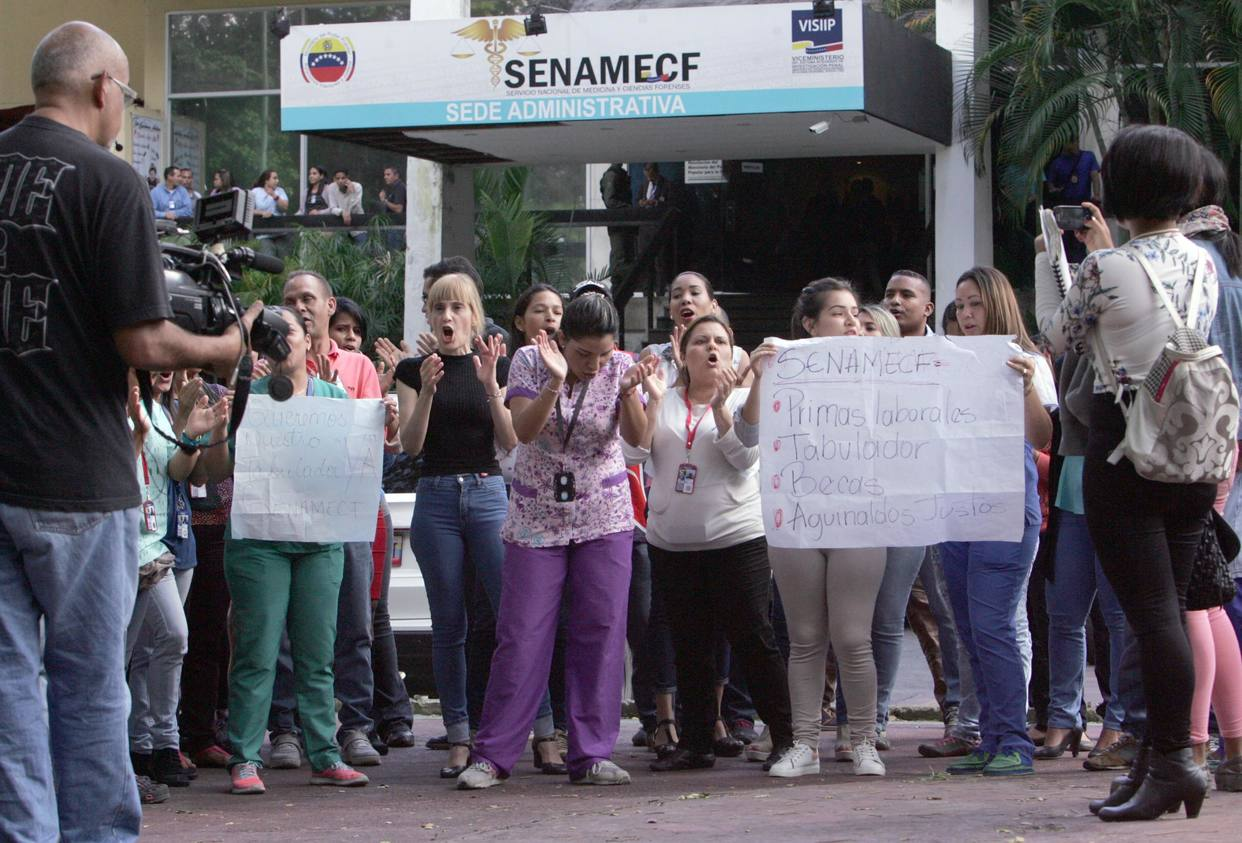
\includegraphics[width=300px]{119.jpg}%
\newline%
%
Operación morrocoy aplicarán los trabajadores adscritos al área de Patología del Servicio Nacional de Medicina y Ciencias Forenses de Bello Monte, debido al incumplimiento de beneficios laborales que incluyen prima de riesgo, actualización del salario luego del último incremento decretado por el Ejecutivo, así como la aplicación de un tabulador profesional luego de la reconversión monetaria. “Éramos uno de los organismos mejor pagados. Ahora nos quitaron nuestras primas y solo devengamos 600 bolívares semanales”, dijo Emily Quevedo, enfermera forense del organismo.%
\newline%
%
La funcionaria destacó que con la llegada de Humberto Ruiz, viceministro del Sistema Integrado de Investigación Penal del Ministerio de Interior, Justicia y Paz, como nuevo director de la morgue de Bello Monte, “acabaría la corrupción dentro del organismo forense. Sabemos que existen nóminas paralelas, nóminas fantasmas. Hay personas que aparecen en el registro de personal y nunca han venido a trabajar. Cobran y por aquí no aparecen”, dijo.%
\newline%
%
La protesta se hizo pública el viernes 9. Trabajadores del área de Patología salieron en horas de la tarde con pancartas y tomaron los espacios de la plaza Auyantepuy, situada entre la avenida Anauco y la Neverí en Colinas de Bello Monte, desde donde exigieron a las autoridades aumento de sueldo y la cancelación de aguinaldos “que sirvan para comprar algo más que seis kilos de carne”, expresaron a través de consignas.%
\newline%
%
La misma acción se replicó ayer con más de 30 trabajadores, entre técnicos, enfermeros forenses y empleados de mantenimiento. Quevedo expresó: “El viceministro envió a personas de prensa adscritas al Senamecf para que nos tomaran fotos y despedirnos del organismo si continuábamos con la protesta, pero aquí estamos, exponemos nuestros rostros porque somos padres y madres de familia que también sufrimos la crisis”, aseguró.%
\newline%
%
Quevedo agregó que hay un brote de enfermedades de piel, tuberculosis y meningitis que amenaza con la salud de los técnicos, médicos y enfermeras forenses desde el mes de enero: “Esto pasa por la falta de insumos para el aseo. Tampoco tenemos material para trabajar los cadáveres, porque nos llega a cuentagotas”.%
\newline%
%
Norelys Gómez, del Departamento de Atención al Ciudadano, dijo que se ha incrementado la deserción laboral debido al descontento por los salarios. También solicitó un cambio en la Gerencia del organismo y la realización de una auditoría de la actual administración.%
\newline%
%
Si los requerimientos exigidos por los trabajadores de Patología Forense no son atendidos, la operación morrocoy se extenderá por 72 horas hasta el miércoles.%
\newline%
%
\end{document}